Wärmetransport ist eine Folge von Temperaturgefällen. Wärme strebt vom warmen Reservoir zum kalten. Das geschiet durch Konvektion, Wärmestrahlung oder Wärmeleitung. In diesem Versuch geht es um die Wärmeleitung in Metallen durch Phononen und frei bewegliche Elektronen -- Beiträge durch die Konvektion und Wärmestrahlung werden vernachlässigt. \\
Für einen Stab der Querschnittsfläche $A$ mit der Wärmeleitfähigkeit $\kappa$ ist die Änderung der Wärme $Q$ in einer Zeitspanne abhängig von der Temperaturänderung bezüglich des Abstandes der Orte, an denen die Temperatur gemessen wurde
\begin{equation}
\text{d}Q = - \kappa A \frac{\partial T}{\partial x} \text{d}t \quad .
\end{equation}
Die eindimensionale Wärmeleitungsgleichung beschreibt die räumliche und zeitliche Entwicklung der Temperatur
\begin{equation}
\frac{\partial T}{\partial t} = \frac{\kappa}{\rho \cdot c} \frac{\partial ^2 T}{\partial x^2} \quad,
\end{equation}
die von den Materialeigenschaften Wärmeleitfähigkeit $\kappa$, Dichte $\rho$ und spezifische Wärme $c$ abhängt.  Der Faktor $\frac{\kappa}{\rho \cdot c}$ stellt dar, wie schnell die Temperaturausbreitung erfolgt und wird auch Temperaturleitfähigkeit genannt. \\
Die Lösung der eindimensionalen Wärmeleitungsgleichung ist abhängig von der Form des Stabes und den Anfangsbedingungen d.h. der Art der Wärmezufuhr. Wird der Stab an einem Ende periodisch erwärmt und abgekühlt, entsteht eine Temperaturwelle $T(x,t)$ entlang des Stabes 
\begin{equation}
T(x,t) = T_\text{max} \cdot \exp\left( - \sqrt{\frac{\omega \rho c}{2 \kappa \right)}} \cdot \cos \left(\omega t - \sqrt{\frac{\omega \rho c}{2 \kappa}}\right) \quad.
\end{equation}
Die Wärmeleitfähigkeit kann aus dem Amplitudenverhältnis einer näher an der Wärmequelle gelegenen Messung $A_\text{nah}$ und einer um $\Delta x$ weiter entfernten Messung $A_\text{fern}$ bestimmt werden
\begin{equation}
\kappa = \frac{\rho  c (\Delta x )^2}{2  \Delta t \ln \left(A_\text{nah} / A_\text{fern}\right)} \quad.
\end{equation}
Die Zeitdifferenz der Amplituden ist $\Delta t$. \newpage
Zum Erwärmen der Stäbe wurde ein \textbf{Peltier-Element} verwendet. Das Peltier-Element heizt nach dem Anlegen einer Spannung auf der einen Seite und kühlt auf der anderen, sodass es sowohl als Wärme- als auch als Kältequelle verwendet werden kann. In einem Peltier-Element sind abwechselnd n- und p-dotierte Halbleiter verbaut und an Lötstellen miteinander verbunden. Elektronen, die sich in den Halbleitern bewegen haben unterschiedliche Energieniveaus. Wenn das Elektron von dem n-dotierten auf den p-dotierten Halbleiter trifft, nimmt es ein höheres Energieniveau an und muss dazu Energie aus der Umgebung aufnehmen -- die Lötstelle kühlt ab. Trifft  das Elektron wieder auf den n-dotierten Halbleiter gibt es Energie ab und die Lötstelle wird heißer.
\begin{figure}
	\centering
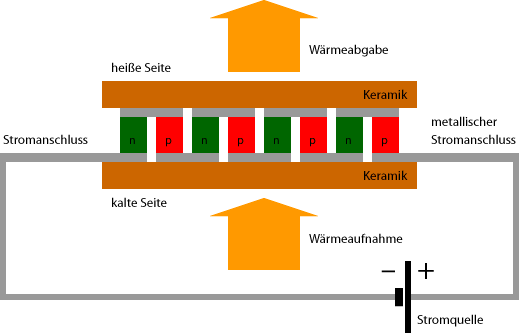
\includegraphics[width=0.75\textwidth]{peltier-element.png}		
\caption{Peltier-Element\footnotemark}
\end{figure}
\footnotetext{Quelle: \url{https://www.energie-lexikon.info/img/peltier-element.png}}


